\chapter{Access Control Techniques}
\label{AccessControlTechniques}
\begin{itemize}
 \item Mandatory Access Control: General (system-determined) access control.
 Specifica di chi può accedere a cosa.
 \item Discretionary Access Control: persone che hanno l'autorizzazione ad
 accedere. Si trova spesso dove l'informazione deve essere classificata
 \item Role-Based Access Control: è la soluzione migliore per i contesti
 organizzativi classici. Essendoci un numero fissato di ruoli per
 l'amministratore di sistema la loro gestione diviene più semplice, piuttosto
che gestire ogni singolo impiegato. Questa realtà è ancora in forte sviluppo.
 \item Physical Access Control: è quell'area legata alla sicurezza fisica, ed è
 legata al CSO ultimamente. Si costituisce di lucchetti, chiavi, ecc...
\end{itemize}


\section{Role-Based Access Control}
\todo{TODO copia tabella}

Prima di mettersi a fare controlli sugli accessi bisogna prima comprendere per
bene quali ruoli sono presenti all'interno dell'azienda (analisi interna).


\section{Military Security Policy}

Si applica una classificazione dell'informazione, che può essere:
\begin{itemize}
 \item Top secret
 \item Secret
 \item Confidential
 \item Non-classified

\end{itemize}

Per evitare l'overclassification si utilizzano i domini: si cercano di mettere
delle persone con determinate competenze nel contesto giusto.
Ad esempio: se un dominio è il nucleare e io non ho competenze a riguardo non
posso accedere a quel dominio.

Un soggetto può accedere ad un oggetto solo se domina la classificazione
dell'oggetto.

\section{Modello Bell-La Padula}

Si è dimostrato che adottando questo modello possiamo avere buone proprietà di
confinamento dell'informazione.

Utilizza il principio di confidenzialità: si può avere accesso in lettura a
tutto ciò che dominiamo. Per la scrittura invece vale il contrario: posso
accedere in scrittura a tutto ciò che mi domina ma non posso scrivere a ciò che
domino. Il tutto viene riassunto in \textit{no read up} e \textit{no write
down}.

Principio di tranquillità: le classi degli oggetti non possono cambiare.

% In che contesto aveva detto sta cosa? Era sempre riguardo Bell-La Padula
La declassificazione risolve il problema del galleggiamento verso l'alto. Avere
troppi documenti top-secret può causare problema. Eseguire una
declassificazione è una procedura costosa, ed è quando il livello di segretezza
di un certo documento viene abbassato.

\section{System Access Control}

Il \textit{System Access Control} si occupa di:
\begin{itemize}
 \item eseguire il log degli eventi
 \item generare report per l'amministrazione di sistema dei tentativi falliti
di accesso, che possono essere anche accidentiali.
\end{itemize}

\section{Application-Level Access Control}

Gli obiettivi del \textit{application-level access control} sono:
\begin{itemize}
 \item creare/cambiare file o struttura del database
 \item autorizzare azioni al livello di:
  \begin{itemize}
   \item applicazione
   \item file
   \item transazione
   \item campo
  \end{itemize}
\item log di accessi alla rete e ai dati
\end{itemize}

\section{Password}
\label{Password}

\subsection{Tutto quello che avreste voluto sapere ma non avete mai osato
chiedere sulle password}

Cos'è una password? Una sequenza arbitraria di caratteri segreta e difficile da
indovinare.

Ancora al tempo di Venezia era presente addirittura una sezione di cifratura
apposita. Oggi, l'NSA è l'istituzione che ha più matematici al mondo.

\subsubsection{Gestione delle password}

Le password servono a discriminare chi ha diritto o no ad accedere al servizio.
Le password nei sistemi vengono solitamente cifrate e salvate, in questa
maniera non è presente la password in chiaro. Per eseguire ciò di solito si
eseguono delle tecniche di \textit{hashing}.

\subsubsection{Difficoltà delle password}

Con una password da N caratteri, in cui ogni carattere può assumere M valori,
abbiamo $N^M$ possibili password.

\subsection{Come creare una buona password}

Le password scelte dagli utenti non sono solitamente forti, ma tendono ad
essere deboli e ripetitive. La bontà di una password dipende anche dalla sua
\textit{entropia}.
Le password solitamente sono simili a quelle di nomi di persone, date di
nascite o numeri di telefono.

\paragraph*{Base words}
Le \textit{base-words passwords} sono password significative dal punto di vista
memnonico che risultano essere difficili da indovinare da un attaccante perchè
per un estraneo risultano come se fossero una combinazione casuale di parole.
È un metodo molto valido per costruire una forte password.

\paragraph*{Facciamo i conti}

Il dizionario inglese ha 170 mila parole, vuol dire che se combiniamo 2 parole
abbiamo 29 miliardi di tentativi per indovinare per password. Il problema è che
le GPU moderne possono provare fino a 40 miliardi di password al giorno.
È possibile attaccare oggi come oggi sistemi molto difesi tramite attacchi di
forza bruta.
$2^{80}$ è il limite teorico oltre il quale un sistema è considerato
inattaccabile. Una password di 10 caratteri con 46 possibili caratteri ha circa
$2^{55}$ possibilità.

\paragraph*{Attacco del dizionario}
Le password sono solitamente deboli all'attacco del dizionario: ovvero sono
password che hanno al loro interno pattern di persone/cose (come ad esempio il
nome di una serie TV o simili). I dizionari al giorno d'oggi sono addirittura
comprabili, e presentano tutte le entry di un determinato campo semantico.
È meglio quindi evitare l'uso di password che abbiano pattern al loro interno.
È meglio la generazione di una password totalmente casuale.

\subsection{Autenticazione a due fattori}

L'autentificazione viene detta forte quando è ad almeno due fattori.
Autenticazione forte vuol dire usare almeno due canali differenti.

Ad esempio al giorno d'oggi durante un'autenticazione bancaria si richiedono
solitamente il proprio codice bancario e un altro codice proveniente da una
chiavetta/sms/token hardware.

Per eseguire una corretta autenticazione il tutto si basa su questi tre punti:
\begin{itemize}
 \item Qualcosa che siamo (impronte biometriche)
 \item Qualcosa che abbiamo (ad esempio una chiavetta)
 \item Qualcosa che sappiamo (ad esempio una password)
\end{itemize}

Per avere un'autenticazione forte devono essere presente almeno due di queste
tecniche. Questo funziona bene perchè almeno due canali devono essere
compromessi da un attaccante per poter ottenere l'accesso.

Una nuova tecnica è anche quella della autorizzazione tramite
geolocalizzazione. Sempre nell'ambito bancario, pagamenti eseguiti a breve
tempo da diverse parti del mondo non vengono autorizzati.

\subsection{Single Sign On}

Vantaggi:
\begin{itemize}
\item una buona password rimpiazza molte password
\item ID consisente tra i sistemi
\item riduce il lavoro degli admin nel setup e per le password dimenticate
\item accesso rapido ai sistemi
\end{itemize}


Il Single Sign On serve per poter accedere a una serie di servizi offerti dal
provider. Con il SSO è il segmento con cui ci si autentica per primi che
fornisce l'autorizzazione anche per le altre applicazioni.
La sicurezza che il SSO offre non è la stessa che la segmentazione dei servizi
offre.
Svantaggi:
\begin{itemize}
\item Single Point of Failure (SPOF) 
\item Lo sviluppo del software è complicato per via di diversi sistemi operativi
\item Implementazione onerosa
\end{itemize}

\todo{AGGIUNGERE LA SLIDE SULL'AUTHENTICATION COMBINATIONS?}
% Da rimuovere?
%\subsection{Multi-factor authenticator}

\subsection{Biometria}

È molto utile per eseguire autenticazioni, ma funziona ancora male in contesti
quali per esempio le riprese di sicurezza.

Chi sei e cosa fai, è suscettibile ad errori.

\begin{itemize}
\item False Rejection Rate: anche detto \textbf{falso negativo}, un reject che
non dovrebbe esserci stato.
\item False Acceptance Rate: anche detto \textbf{falso positivo}, un accept
quando non avrebbe dovuto esserci.
\item Failure to Enroll Rate: numero di utenti che non sono riusciti a
registrarsi correttamente
\end{itemize}

\subsubsection{Metodi migliori per l'autenticazione}

\begin{figure}[H]
 \centering
 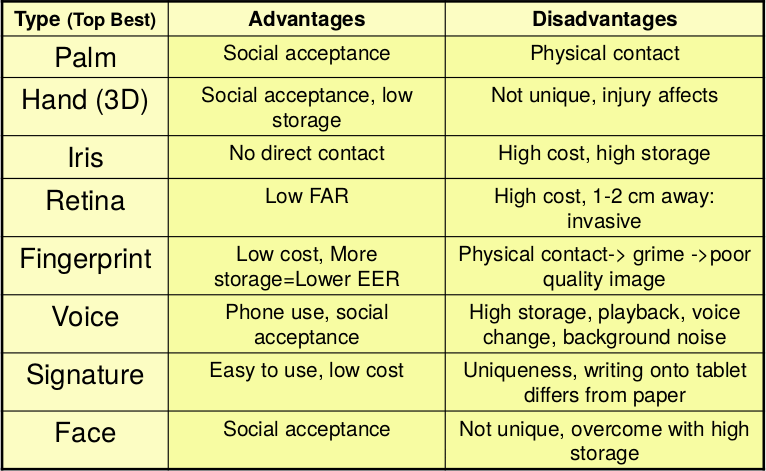
\includegraphics[scale=0.425]{best_biometrics_table}
 \caption{Confronto tra le varie biometrie rispetto a tempo di risposta e EER (\emph{Equal Error Rate}) più basso. }
\end{figure}


\subsubsection{Biometric Info Management \& Security (BIMS) Policy}

\begin{itemize}
 \item Procedure di identificazione e autenticazione
 \item Backup delle autenticazioni (es. non chiedere l'autenticazione ogni
 volta)
 \item Trasmissione/conservazione sicura dei dati biometrici
 \item Sicurezza fisica dell'hardware
 \item Test di valutazione
\end{itemize}

I dispositivi per la cattura del viso per esempio stanno in aree aperte, e se
un attaccante è in grado di manomettere il dispositivo ha la possibilità di
inserire un dispositivo di acquisizione personale, per poter registrare i dati
e ottenerli in maniera non autorizzata. In questa maniera l'attaccante è in
grado di eseguire un furto d'identità. Questi strumenti dovrebbero essere posti
in aree controllate, cosa che spesso non succede. È importante che l'integrità
di questi strumenti venga manetenuta.

\subsection{Verifiche di un IS Auditor}
\begin{itemize}
 \item Verificare che ci siano delle procedure
 \item Che siano implementate
 \item che i processi seguano il pattern del \textit{need to know}
 \item security awareness
 \item L'owner e il custode devono sapere di essere responsabili di quello che
 fanno e
 \item Security Adimistrator deve forni
 \item I meccanismi di sicurezza devono essere aggiornati e consistenti con la
 realtà
 \item I servizi amministrativi devono essere consistenti, e devono provvedere
 sicurezza fisica e logica
\end{itemize}

% ESERCIZI
\section{Esercizi}

Gli esercizi sono disponibili nella sezione apposita, in \ref{EsPass}
